It is well understood that the way to achieve peak performance/lowest latency inference of a DNN is to linearize the \commnt{cite ther nersc roofline paper}{control flow graph} (i.e., remove branches) and flatten the \commnt{cite torsten}{dataflow graph as much as possible} (execute as many operations in parallel as possible).
For intermediate level representations of a DNN (e.g., loops) this corresponds, roughly, to loop fusion followed by loop unrolling followed by store-load forwarding or, alternatively, wholly promoting stores-loads to registers.
In principle, we could rely on MLIR for each of these, or alternatively MLIR for loop fusion and LLVM for loop unrolling, store-load forwarding, and register promotion.
The chief impediment to relying on these general purpose compilers for our needs is the complexity and sophistication of the algorithms used to perform each phase of the translation in an automated way.
For example, in MLIR, the loop fusion pass checks that memory independence constraints are satisfied for all pairs of stores and loads in each loop nest to be fused.
That means unroll and fuse optimizations (\commnt{\url{https://www.clear.rice.edu/comp512/Lectures/Papers/1971-allen-catalog.pdf}}{alternatively known as unroll and jam}) take increasingly longer as one experiments with larger and larger unroll thresholds (unroll all loops with trip count less than or equal to the threshold).
For store-load forwarding, for each load that follows a store, the compiler must check whether the store and the load access the same location in memory, and further verify that there are no intervening stores to the same memory address; for stores in the body of a loop, this requires solving the constraint system discussed in <section background on memory dependencies>.

For general purpose programs this is an acceptable cost, especially given that most development is done without aggressive optimization in order to get fast build times in order to iterate on the logic of the program (leaving the aggressive optimization compilations for release ready builds).
For us, given that the logic of BraggNN is fixed (having already been iterated on), and given that we are in fact searching the design space for optimal low-level representations of the DNN, the runtimes of these algorithms are prohibitive (taking on the order of hours and sometimes days to complete).
Moreover, often their rigor and conservatism are unnecessary given a high-level understanding of the structure of BraggNN; for example, in the case of fully unrolling a convolution and forwarding from the stores during initialization to the loads during accumulation, the region within which the forward is safe is clear from the semantics of convolutions (stores can be forwarded to their first load and subsequent stores can be forward to immediately subsequent loads).
The loop indices and corresponding memory addresses for these safe store-load forwards are very easy to compute analytically ahead of time (even in the presence of complications such as strided tensors).

In order to avoid these enormously costly and unnecessarily complex optimization passes, we completely omit them.
Instead, we do not lower BraggNN past the scf dialect, and instead implement an \commnt{check this name with karthik}{abstract interpreter, which }performs the unrolling blindly (i.e., without verifying constraints) but correctly, i.e., in such a way that the unrolled loops do not perform invalid stores/loads.
In addition to efficiently unrolling loop nests, our abstract interpreter promotes almost all stores-loads to registers, since, in the context of FPGAs, registers are plentiful.
Furthermore, since BraggNN is a relatively small DNN, we inline absolutely all of the weight tensors as constants and perform constant propagation.
This completely eliminates all logic (integer arithmetic) related to calculating memory offsets, a non-trivial reduction in instruction count and design complexity (see figure <figure> for reduction in instruction count).
Finally, we fuse sequences of multiplications and additions into single operation fused-multiply-add.
The reinterpreted semantics implemented by our abstract interpreter are presented in figure <figure>.

\commnt{place holder semantics}{
  \begin{figure}
    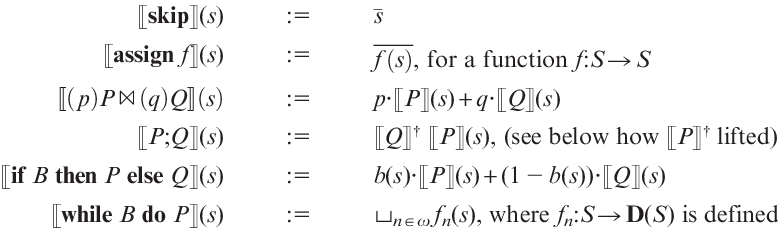
\includegraphics[width=\columnwidth]{figures/semantics.png}
    \caption{This is a placeholder.}
  \end{figure}
}  

In addition to reducing the runtime of the MLIR frontend, our abstract interpreter simplifies the LLVM IR that we could pass to Vitis, and thus, in theory reduces its workload as well.
In actuality, even if one waits for the frontend compiler passes to complete (i.e., MLIR or LLVM), Vitis will rerun the same or similar passes without any intervention by the user, on behalf of the user, as part of its default optimization/transformation pipeline.
In addition to the unnecessary passes, Vitis takes an inordinate amount of time to schedule the large number of operations that comprise BraggNN when fully unrolled (even after eliding unnecessary operations such as memory offset arithmetic).

Recall that the crucial task which Vitis HLS fulfills is the scheduling of operations during each clock cycle, in such a way that they respect the dataflow graph, and constructing the corresponding FSM.
In general, for complex programs, this is indeed a difficult task, necessitating formulating the scheduling problem (as described in background) and solving it using either an LP solver or some heuristic.
But in the case of BraggNN, and in fact many DNNs, where the dataflow is very regular and where parallel execution is only bounded by the number of DSPs (since we eliminate the need for BRAMs by using only registers), it is straightforward to construct the optimal schedule based solely on a topological sort of the operations.
In fact, by performing the scheduling ourselves, we can exercise more control over DSP usage.
Thus, we schedule using the maximum number of DSPs possible during each state of the FSM/schedule, whereas Vitis attempts to make conservative use of DSPs, which leads to excessive LUT usage for muxing (as discussed in background section <....>); see figure <...> for a comparison the LUT usage using our scheduling algorithm versus Vitis' scheduling algorithm.
One thing to note here is that even just performing this scheduling (even without any of the unnecessary IR optimization passes) becomes costly (in terms of runtime) for the larger scalings of BraggNN, where we need to schedule upwards of 1E6 operations.
To ameliorate these costs we implement a \commnt{\url{https://link.springer.com/book/10.1007/978-3-030-25209-0}}{parallelized topological sort}.
Thus, we build our schedule, bounded only by the number of available DSPs, extract the control FSM, and generate the corresponding RTL (Verilog).

In addition to being able to exercise precise control over total DSP usage, we are able to exercise more precise control over how the DSPs are configured; Vitis, \commnt{\url{https://support.xilinx.com/s/question/0D52E00006hpMZQSA2/vitis-hls-cannot-invoke-dspfp32-maddmacc-mode-for-versal?language=en_US}}{due to a current bug}, cannot infer fused-multiply-adds ($a \times b + c$), whereas we can directly instantiate such operations.
Thus, we instantiate the maximum number of fused-multiply-adds and map all arithmetic operations to these units.
Note that since FPGAs cannot be reconfigured at runtime, in order for this to be feasible, we must normalize all arithmetic operations in BraggNN to be in terms of $a \times b + c$.
For multiplications (setting $c = 0$) and additions (setting $b = 1$) this is straightforward.
For subtractions, we can preprocess the \commnt{yes this is a real word}{subtrahend} by flipping the sign bit (and setting $b = 1$).
Division is the only primitive operation that presents a serious challenge to normalization in this way.
To normalize division we exploit the fact that aliasing floating point to an integer implements\commnt{\url{https://en.wikipedia.org/wiki/Fast_inverse_square_root\#Aliasing_to_an_integer_as_an_approximate_logarithm}}{ an approximate binary logarithm}; we use this property to approximate the inverse (of a floating point number) and then perform division by multiplication by that inverse.
In our experiments (and \commnt{\url{https://link.springer.com/chapter/10.1007/978-0-387-72258-0_14}}{prior work}) this approximation incurs only a $\sim 4\%$ difference in accuracy per division.

Finally, we experiment with alternative bitwidth implementations of IEEE754 single precision floating point.
Over the course of inspecting the sample data that BraggNN was trained on, we observe that the sample data does not use a full 8 bit exponent:  
\begin{figure}
  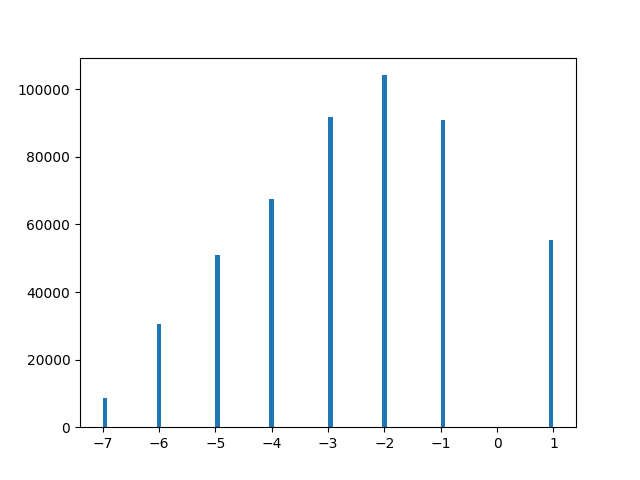
\includegraphics[width=\columnwidth]{figures/exp_bits}
  \caption{This is a placeholder.}
\end{figure}
To this end, we employ the \commnt{\url{https://ieeexplore.ieee.org/document/8877424}}{FloPoCo generator of arithmetic }cores to generate IEEE754 floating point fused multiply adds with 3 bits for the exponent (and 23 bits for the mantissa).
This produces floating point arithmetic cores that use fewer registers and have smaller wire delays.

Thus in summary, inspired by the FloPoCo project, our design methodology can be best described as \emph{computing just right}, i.e., just the right amount of compute and abstraction for the task at hand, no more no less, and we demonstrate that such a methodology produces peak performance (minimum inference latency).